\documentclass[12pt]{article}


\usepackage{amsmath, amssymb}
\usepackage{verbatim}
\usepackage{tikz} 
\usetikzlibrary{shapes}
\usetikzlibrary{arrows}
\usetikzlibrary{positioning}
\usetikzlibrary{patterns}
\usetikzlibrary{calc}
\usetikzlibrary{shapes.geometric}
\usetikzlibrary{backgrounds,calc,shadings,shapes.arrows,shapes.symbols,shadows}

\usepackage[margin=1.4in,footskip=.25in]{geometry}


\tikzset{red/.style={rectangle, draw,fill=red, font=\ttfamily, minimum width =10pt, minimum height=10pt}}
\tikzset{grn/.style={rectangle, draw, fill=green, font=\ttfamily, minimum width =10pt, minimum height=10pt}}
\tikzset{blk/.style={font=\ttfamily, minimum width =10pt, minimum height=10pt}}

\tikzstyle{input}=[
        draw,
        trapezium,
        trapezium left angle=60,
        trapezium right angle=120,
        inner sep=10pt,
        fill=white!25
]
\tikzstyle{output}=[
        draw,
        trapezium,
        trapezium left angle=60,
        trapezium right angle=120,
        inner sep=10pt,
        fill=white!25
]
\tikzstyle{debutfin}=[
	ellipse,
	draw,
	text=black,
	inner sep=10pt
]
\tikzstyle{instruct}=[
	rectangle,
	draw,
	fill=white!50,
	inner sep=10pt
]
\tikzstyle{test}=[
	diamond, 
	aspect=1,
	thick,
	draw=black,
	fill=white!50,
	text=black
]
\tikzstyle{es}=[
	rectangle,
	draw,
	rounded corners=4pt,
	fill=white!25,
	inner sep=10pt
]
%styledesflèches
\tikzstyle{suite}=[
	->,
	>=stealth,
	thick,
	rounded corners=4pt
]


\tikzstyle{subj} = [
	circle, 
	minimum width=8pt, 
	fill, 
	inner sep=10pt
]

\tikzstyle{obj}  = [
	circle, 
	minimum width=8pt, 
	draw, 
	inner sep=20pt
]

\tikzstyle{dc}   = [
circle, 
minimum width=8pt, 
draw, 
inner sep=10pt, 
path picture=
	{
	\draw 
		(path picture bounding box.south east) -- 
		(path picture bounding box.north west) 
		(path picture bounding box.south west) -- 
		(path picture bounding box.north east);
	}
]



\tikzset{
  pivot/.style={
    draw, 
    regular polygon, 
    regular polygon sides = 3, 
    fill = blue!30, 
    node distance = 1cm, 
    minimum height = 2em,
    inner sep=10pt, 
  }
}





\makeatletter
\pgfkeys{/pgf/.cd,
  parallelepiped offset x/.initial=2mm,
  parallelepiped offset y/.initial=2mm
}


\pgfdeclareshape{parallelepiped}
{
  \inheritsavedanchors[from=rectangle] % this is nearly a rectangle
  \inheritanchorborder[from=rectangle]
  \inheritanchor[from=rectangle]{north}
  \inheritanchor[from=rectangle]{north west}
  \inheritanchor[from=rectangle]{north east}
  \inheritanchor[from=rectangle]{center}
  \inheritanchor[from=rectangle]{west}
  \inheritanchor[from=rectangle]{east}
  \inheritanchor[from=rectangle]{mid}
  \inheritanchor[from=rectangle]{mid west}
  \inheritanchor[from=rectangle]{mid east}
  \inheritanchor[from=rectangle]{base}
  \inheritanchor[from=rectangle]{base west}
  \inheritanchor[from=rectangle]{base east}
  \inheritanchor[from=rectangle]{south}
  \inheritanchor[from=rectangle]{south west}
  \inheritanchor[from=rectangle]{south east}
  \backgroundpath{
    % store lower right in xa/ya and upper right in xb/yb
    \southwest \pgf@xa=\pgf@x \pgf@ya=\pgf@y
    \northeast \pgf@xb=\pgf@x \pgf@yb=\pgf@y
    \pgfmathsetlength\pgfutil@tempdima{\pgfkeysvalueof{/pgf/parallelepiped
      offset x}}
    \pgfmathsetlength\pgfutil@tempdimb{\pgfkeysvalueof{/pgf/parallelepiped
      offset y}}
    \def\ppd@offset{\pgfpoint{\pgfutil@tempdima}{\pgfutil@tempdimb}}
    \pgfpathmoveto{\pgfqpoint{\pgf@xa}{\pgf@ya}}
    \pgfpathlineto{\pgfqpoint{\pgf@xb}{\pgf@ya}}
    \pgfpathlineto{\pgfqpoint{\pgf@xb}{\pgf@yb}}
    \pgfpathlineto{\pgfqpoint{\pgf@xa}{\pgf@yb}}
    \pgfpathclose
    \pgfpathmoveto{\pgfqpoint{\pgf@xb}{\pgf@ya}}
    \pgfpathlineto{\pgfpointadd{\pgfpoint{\pgf@xb}{\pgf@ya}}{\ppd@offset}}
    \pgfpathlineto{\pgfpointadd{\pgfpoint{\pgf@xb}{\pgf@yb}}{\ppd@offset}}
    \pgfpathlineto{\pgfpointadd{\pgfpoint{\pgf@xa}{\pgf@yb}}{\ppd@offset}}
    \pgfpathlineto{\pgfqpoint{\pgf@xa}{\pgf@yb}}
    \pgfpathmoveto{\pgfqpoint{\pgf@xb}{\pgf@yb}}
    \pgfpathlineto{\pgfpointadd{\pgfpoint{\pgf@xb}{\pgf@yb}}{\ppd@offset}}
  }
}
\makeatother



\tikzstyle{pc1}   = [
parallelepiped, 
minimum width=12pt, 
text width=12pt, 
inner sep=12pt, 
draw, 
line width=2pt, 
path picture=
	{
	\draw (-1,-1) -- ++(1,-2);
	}
]




\tikzset{
  ports/.style={
    line width=0.3pt,
    top color=blue!20,
    bottom color=blue!20
  },
  rack switch/.style={
    parallelepiped,fill=white, draw,
    minimum width=1.25cm,
    minimum height=0.25cm,
    parallelepiped offset x=2mm,
    parallelepiped offset y=1.25mm,
    xscale=-1,
    path picture={
      \draw[top color=gray!5,bottom color=gray!40]
      (path picture bounding box.south west) rectangle 
      (path picture bounding box.north east);
      \coordinate (A-west) at ([xshift=-0.2cm]path picture bounding box.west);
      \coordinate (A-center) at ($(path picture bounding box.center)!0!(path
        picture bounding box.south)$);
      \foreach \x in {0.275,0.525,0.775}{
        \draw[ports]([yshift=-0.05cm]$(A-west)!\x!(A-center)$)
          rectangle +(0.1,0.05);
        \draw[ports]([yshift=-0.125cm]$(A-west)!\x!(A-center)$)
          rectangle +(0.1,0.05);
       } 
      \coordinate (A-east) at (path picture bounding box.east);
      \foreach \x in {0.085,0.21,0.335,0.455,0.635,0.755,0.875,1}{
        \draw[ports]([yshift=-0.1125cm]$(A-east)!\x!(A-center)$)
          rectangle +(0.05,0.1);       
      }
    }
  },
  server/.style={
    parallelepiped,
    fill=white, draw,
    minimum width=0.35cm,
    minimum height=0.75cm,
    parallelepiped offset x=3mm,
    parallelepiped offset y=2mm,
    xscale=-1,
    path picture={
      \draw[top color=gray!5,bottom color=gray!40]
      (path picture bounding box.south west) rectangle 
      (path picture bounding box.north east);
      \coordinate (A-center) at ($(path picture bounding box.center)!0!(path
        picture bounding box.south)$);
      \coordinate (A-west) at ([xshift=-0.575cm]path picture bounding box.west);
      \draw[ports]([yshift=0.1cm]$(A-west)!0!(A-center)$)
        rectangle +(0.2,0.065);
      \draw[ports]([yshift=0.01cm]$(A-west)!0.085!(A-center)$)
        rectangle +(0.15,0.05);
      \fill[black]([yshift=-0.35cm]$(A-west)!-0.1!(A-center)$)
        rectangle +(0.235,0.0175);
      \fill[black]([yshift=-0.385cm]$(A-west)!-0.1!(A-center)$)
        rectangle +(0.235,0.0175);
      \fill[black]([yshift=-0.42cm]$(A-west)!-0.1!(A-center)$)
        rectangle +(0.235,0.0175);
    }  
  },
  computer/.style={
    parallelepiped,
    fill=white, draw,
    minimum width=1cm,
    minimum height=0.75cm,
    parallelepiped offset x=1mm,
    parallelepiped offset y=1mm,
    xscale=-1,
    path picture={
    \draw[top color=gray!5,bottom color=gray!40]
      (path picture bounding box.south west) rectangle 
      (path picture bounding box.north east);
      \coordinate (A-center) at ($(path picture bounding box.center)!0!(path picture bounding box.south)$);
      \coordinate (A-west) at ([xshift=-1cm,yshift=.65cm]path picture bounding box.west);
      \draw[ports]([yshift=-1cm]$(A-west)!0!(A-center)$)
        rectangle +(.8,.6);
      %\draw[ports]([yshift=0.01cm]$(A-west)!0.085!(A-center)$)
        rectangle +(0.15,0.05);
      %\fill[black]([yshift=-0.35cm]$(A-west)!-0.1!(A-center)$) rectangle +(0.235,0.0175);
      %\fill[black]([yshift=-0.385cm]$(A-west)!-0.1!(A-center)$) rectangle +(0.235,0.0175);
      %\fill[black]([yshift=-0.42cm]$(A-west)!-0.1!(A-center)$) rectangle +(0.235,0.0175);
    }  
  },
}











\begin{document}


\begin{comment}


\begin{tikzpicture}
	\node[es] (a) at (0,0) {};
\end{tikzpicture}

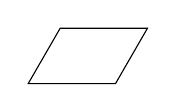
\begin{tikzpicture}
	\node[input] (a) at (0,0) {};
\end{tikzpicture}



\begin{tikzpicture}
	\node[debutfin] (a) at (0,0) {};
\end{tikzpicture}

\begin{tikzpicture}
	\node[instruct] (a) at (0,0) {};
\end{tikzpicture}


\begin{tikzpicture}
	\node[test] (a) at (0,0) {};
\end{tikzpicture}


\begin{tikzpicture}
	\node[subj] (a) at (0,0) {};
\end{tikzpicture}


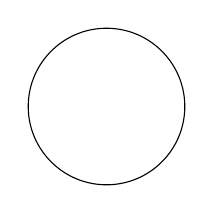
\begin{tikzpicture}
	\node[obj] (a) at (0,0) {};
\end{tikzpicture}



\begin{tikzpicture}
	\node[dc] (a) at (0,0) {};
\end{tikzpicture}

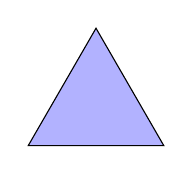
\begin{tikzpicture}
	\node[pivot] (a) at (0,0) {};
\end{tikzpicture}


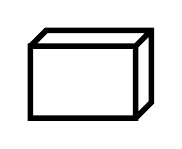
\begin{tikzpicture}
	\node[pc1] (a) at (0,0) {};
\end{tikzpicture}
\end{comment}


%\path[->] (zb) edge node[swap]  {$t$} (xb);
%\path[->] (xb) edge node {$\alpha$} (yb);
%\path[->] (xb) edge[bend left=60] node {$\alpha$} (yb);







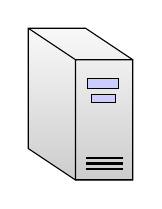
\begin{tikzpicture}
\node[server,scale=2] (server1) at (0,0) {};
\end{tikzpicture}



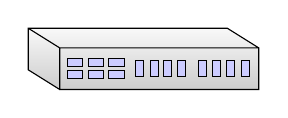
\begin{tikzpicture}
\node[rack switch,scale=2] (server1) at (0,0) {};
\end{tikzpicture}



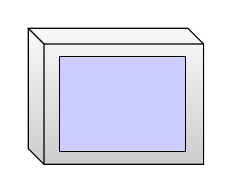
\begin{tikzpicture}
\node[computer,scale=2] (server1) at (0,0) {};
\end{tikzpicture}



\end{document}